%
% The points that I want to cover are the following:
%
% \begin{itemize}
%   \item Building the network from the bioinformatics data and clustering.
%   \item Manipulation of the network: translation and scaling.
%   \item Locomotion and ergonomics used in the VR environment.
%   \item Changing from the blood network to the biopsy network and viceversa.
%   \item Filtering genes in the network using gene sets that represent signatures of cellular pathways which are often dis-regulated in cancer.
% \end{itemize}

%In order to explore the network, several features have been implemented with the purpose of enhance the experience of the visualization process. For example the user has the possibility to move around the network by teleporting to a different place. It is also possible to translate the network and scale it, allowing the user have a better view of the data. The user can also point at a node using the controller to show the name corresponding to that gene or node. Another feature is about entering into a menu where the user can filter the network according to gene sets that represent signatures of cellular pathways which are often dis-regulated in cancer. And finally it is possible also to switch the network from a blood dataset to a biopsy dataset and viceversa.

%The genes nodes in the network and are represented as squared dots and the relationships are represented with lines between them. In Figure \ref{fig:bignet_vr} we can see an example of the application running.

BigNet VR is a virtual reality application for the interactive visualization of large-scale networks in a 3D space. The networks are represented using nodes and connections between them. In order to explore the data, the user can walk around, scale the network, move it around, filter the nodes using a 2D interface and also interact with the nodes to get more information about them. In Figure \ref{fig:bignet_vr} we can see an example of the application running.

BigNet VR works with a dataset that contains the information of the nodes and relationships of the network. This dataset needs to be obtained from an external source or application. Once we have our dataset we can load it to the application and then run BigNet VR using a Head Mounted Display or HMD for VR. Finally we can explore the network and interact with it to visualize the dataset in a VR experience.

The implementation of BigNet VR is done in Unity, a cross-platform game engine. This engine is used for a wide range of applications, especially for the development of videogames in 3D and 2D, VR applications and engineering solutions. The programming language used to develop the application inside Unity is C\#. We also used VRTK, a VR toolkit to build VR solutions in Unity. As for the VR hardware, we used an Oculus Quest headset. This type of headset is an oll-in-one HMD, which means that it doesn't need to be connected to a PC to run an application, it can be run inside the hardware of the headset itself. However during the development process, the headset needs to be connected to the PC and the application can be run directly from Unity.

For this chapter we will use dataset examples from MIxT to illustrate the concepts in this chapter. MIxT is a web application that is used for the visualization of bioinformatic data\cite{fjukstad_dumeaux_olsen_lund_hallett_bongo_2017}\cite{dumeaux_fjukstad_interactions_tumor_blood} and the datasets used here contain genetic information about a woman with breast cancer. There are in total 2 datasets, the first one is from a blood sample and the second one is from the tumor sample. In Figure \ref{fig:bignet_vr} we can see an example of the application running using the blood dataset from MIxT.

\begin{figure}[h!]
    \setlength{\tempheight}{15ex}
    \centering
    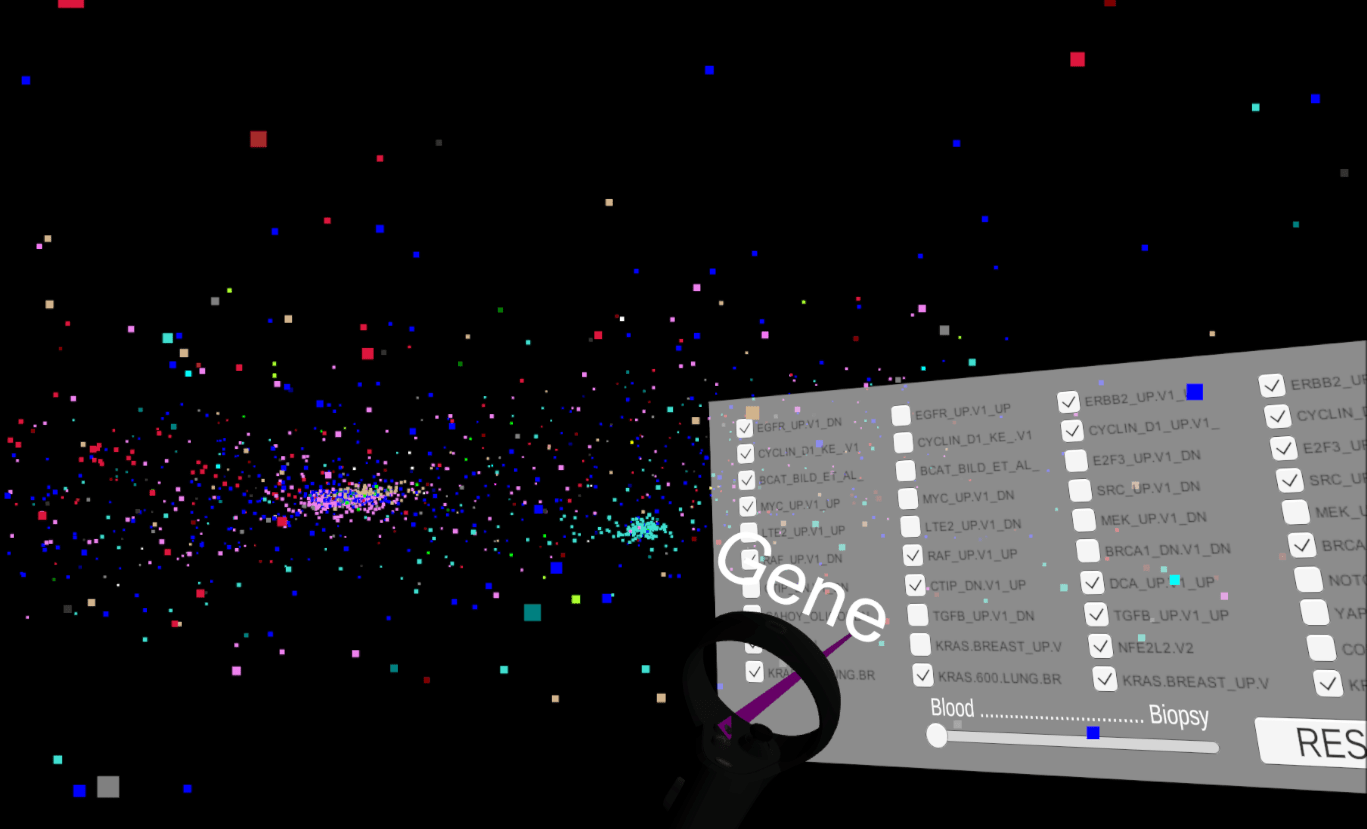
\includegraphics[width=\textwidth]{bignet_vr}
    \caption{BigNet VR. Example of the application running on a Oculus Quest.}
    \label{fig:bignet_vr}
\end{figure}

\section{Visualization and interaction with the network}
Virtual reality headsets offer a rich inmmersive experience. It's not only about inmersing the user into a 3D environment, but also giving the user the possibility to interact with the environment itself. This makes it possible to build complex VR applications where the user can do almost anything in a virtual world. Some examples of what it is possible to do in a VR application are moving around by teleporting to a different spot, grabbing objects, interact with the environment, 2D interfaces and menus and interact with them, etc. In this section we will explain the techniques that we have implemented to visualize and interact with the network. These techniques correspond to how the user can move around in the network and how the user can manipulate it.

Oculus Quest is an all-in-one VR headset and so it doesn't need a PC nor wires to run the applications. Apart from the headset it comes with 2 controllers, one for each hand. These controlers have inputs as buttons, thumbsticks and triggers that can be used to activate actions in the VR application. We have used some of these inputs available in the controllers in BigNet VR and mapped them to different actions that allow the user interact with the network and the environment. In Figure \ref{fig:oculus_quest_inputs} we can see which action correspond each input from the controllers.

\begin{figure}[h!]
    \centering%
    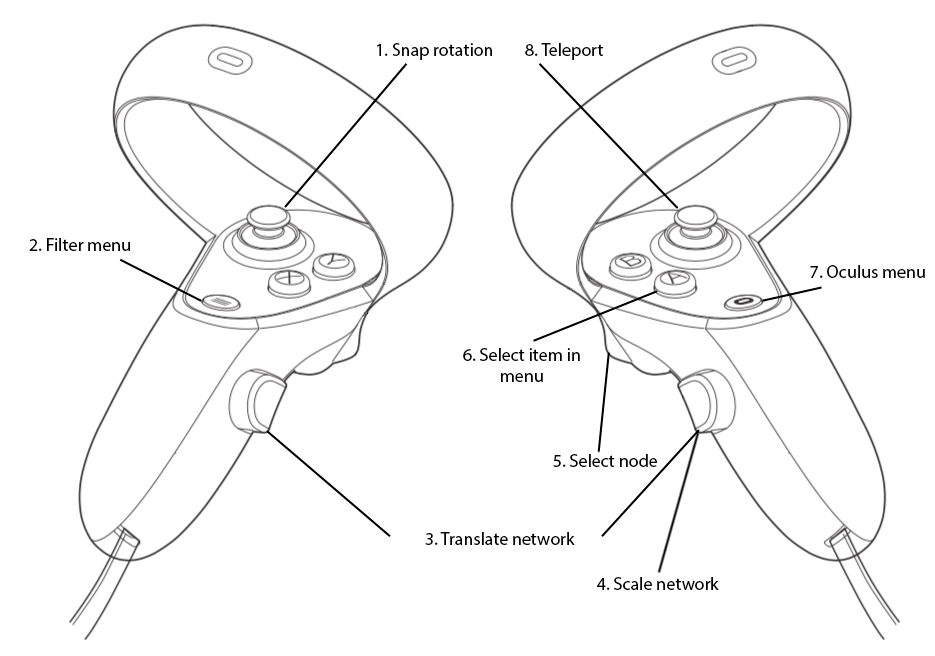
\includegraphics[width=\textwidth]{oculus_quest_inputs}
    \caption{Mapping of the Oculus Quest controllers for the different actions implemented in BigNet VR. 1. Snap rotation. 2. Filter menu. 3. Scale environment. 4. Translate environment. 5. Select item in menu. 6. Oculus menu. 7. Teleport. Adapted figure from Oculus developer's page\cite{oculus_inputs}.}
    \label{fig:oculus_quest_inputs}
\end{figure}%

\subsection{Locomotion}
Locomotion is one of the most important ways of interaction in virtual reality experiences. It can be defined as a self-proppelled movement in virtual environments. Even though moving around is not the main goal in most of VR applications, it is an important aspect for the user's perspective in order to move the user's viewpoint in the virtual world.

Locomotion can have an strong influence in the user's experience. A poorly designed locomotion technique can reduce the user's immersion and even introduce motion sickness, which is related to the movement that the locomotion technique produces. HMDs like Oculus Quest allow the users to control the position and the orientation of the viewpoint by moving their heads and walking. However large virtual environments such as BigNet VR needs a big physical tracked area which cannot be covered by just walking around. It is for this reason that we need to use a locomotion technique that makes it possible to move around without the having to walk\cite{locomotion_technique}.

The locomotion technique that we use in BigNet VR is called teleportation. It consists in choosing a spot on the floor were we want to teleport to. To do this the user has to move forward the joystick from the right controller (see input 7. Teleport from Figure \ref{fig:oculus_quest_inputs}). In addition it is possible to choose which direction the user will face once the teleportation is done. To do this we just need to rotate the same joystick to the desired direction. Once the user releases the joystick, a black flash will show followed by the new position. This black flash is very important when implementing some techniques because it prevents from producing motion sickness and disorientation.

In Figure \ref{fig:teleportation} we can see an example of how the teleportation technique is used in BigNet VR. As we can see, a parabolic arc is shown as if we are throwing an object to the spot where we want to teleport. A round green circle is also shown on the floor on the place where we will teleport. This includes also an arrow, indicating the direction that we will face once we are teleported.

\begin{figure}[h!]
    \centering%
    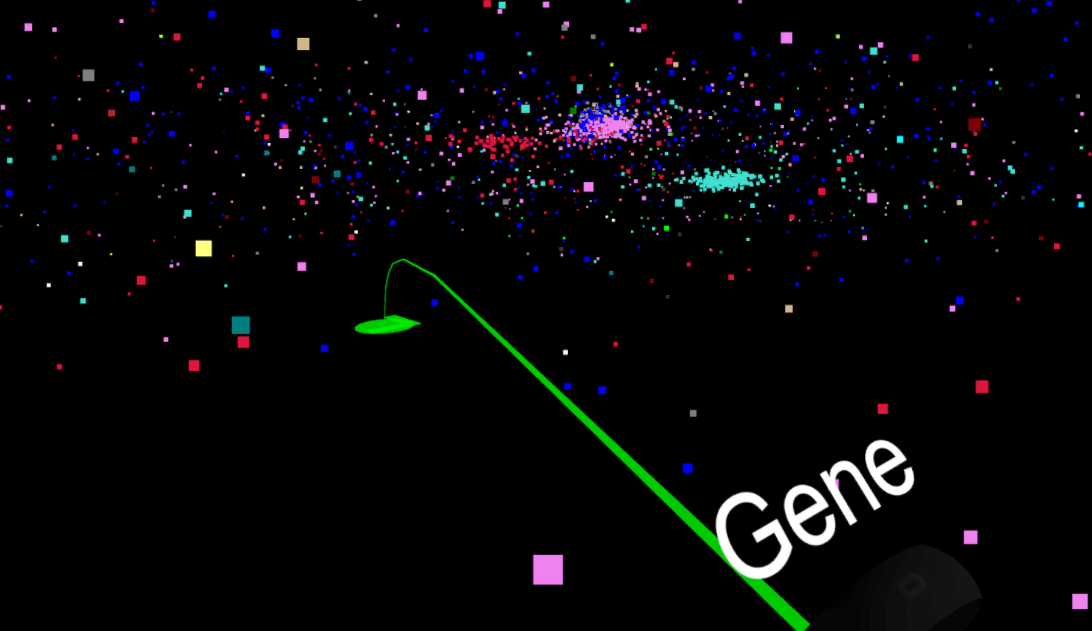
\includegraphics[width=\textwidth]{teleportation2}
    \caption{Teleportation technique. The user can use the jystick from the right controller to teleport to a different spot. To choose the spot a parabolic arc will appear.}
    \label{fig:teleportation}
\end{figure}%

\subsection{Translation of the network}
By teleporting to different places in the environment we allow the user see the network from different perspectives. However it is also interesting being able to move the network and specially move in a precise way so that the user has more control over it. The user might for instance be able to see the network or a specific node or cluster from above or also from below. To do this we have implemented a functionality to translate the network to wherever we want.

In order to translate the network in BigNet VR, the user just needs to press on the 4. Translate environment button from the right controller as shown in \ref{fig:oculus_quest_inputs}. Then the user needs to keep holding this button down and move the hand to the direction to which the user wants the network to move to. This is a very intuitive approach because it feels like we are just pulling from a rope that is connected to the network so we just need to move it to the direction we want without involving a lot of learning for this process.

\begin{figure}[h!]
    \centering%
    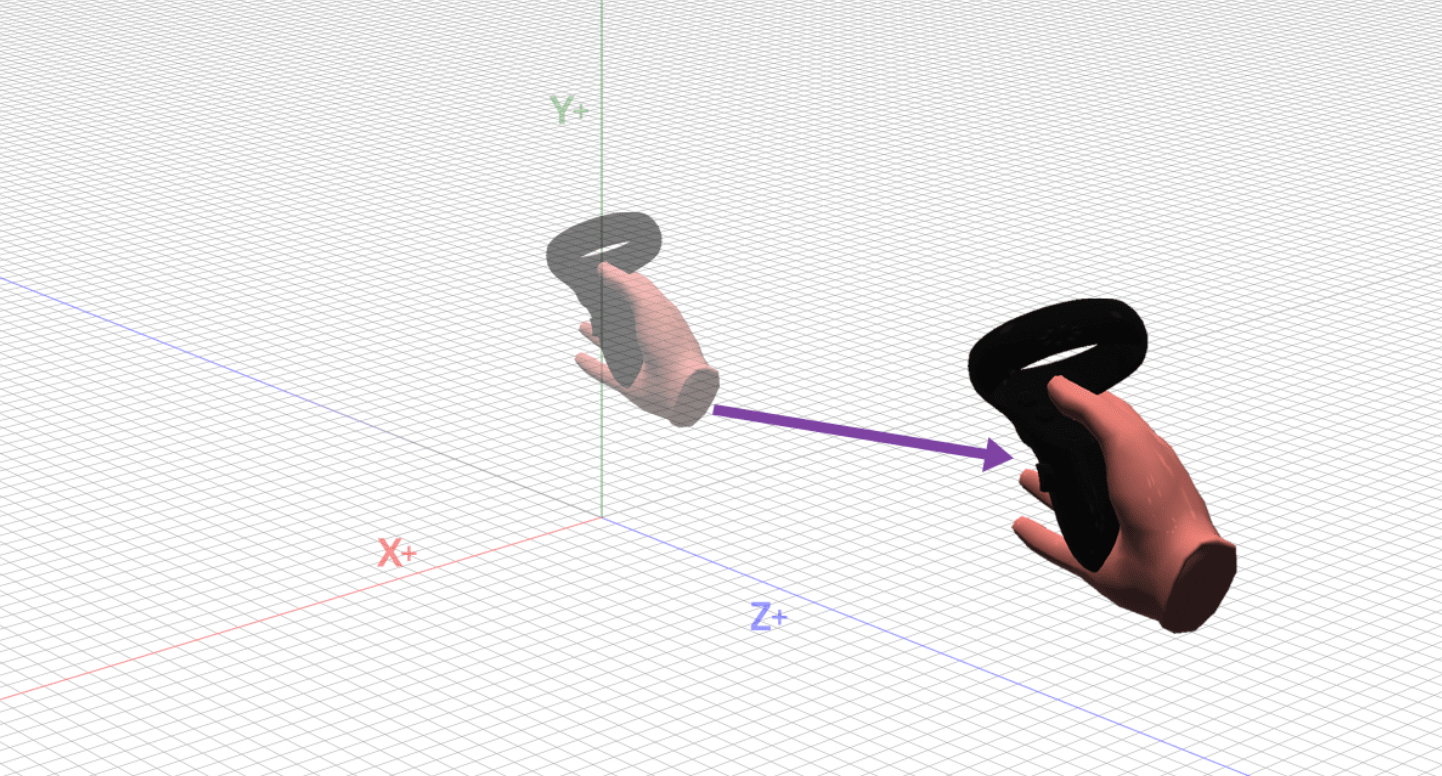
\includegraphics[width=\textwidth]{translation}
    \caption{Translation of the network functionality. The user holds the translation button on the Oculus controller and moves the hand to the direction where he or she wants the network to translate.}
    \label{fig:translation}
\end{figure}%

\subsection{Zooming in the network}
When exploring a big network with hundreds of nodes, sometimes the information can be too crowded. In our example dataset that we use in BigNet VR, there are some clusters of nodes that have too many nodes close to each other and it gets very hard to visualize them properly. A way to cope with this problem is for instance by "zooming" in the part of the network that we want to explore better. We implement then a scaling functionality that makes the network bigger or smaller and so simulating a zooming action.

The way we implemented the zooming functionality in BigNet VR is by using the side buttons with the name "3. Scale environment" shown in Figure \ref{fig:oculus_quest_inputs}. In the first place the user needs to press and hold this button from both right and left controllers and in the second place the user needs to expand or contract the arms, as if we were streching out or contracting the network itself. This is also an intuitive acction to do since the user might think that he or she is actually stretching the network with the hands.

In Figure \ref{fig:scaling} we an see a visual example of how the zooming works using the Oculus controllers. In this example the user is stretching the hands out in order to make the network bigger. The user starts in a intial position, then holds the zooming buttons from both controllers and then moves the hands out. If we wanted to make the network smaller we would have to do the opposite action, by contracting the hands to the inside.

\begin{figure}[h!]
    \centering%
    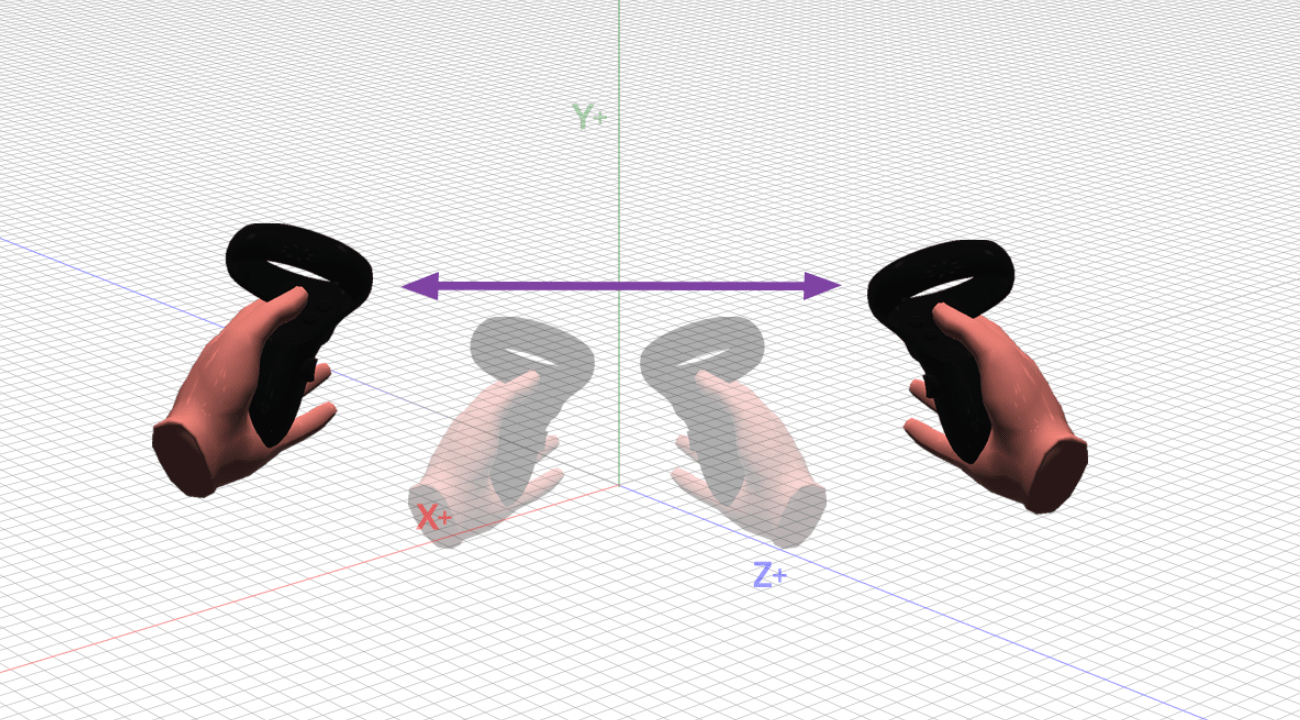
\includegraphics[width=\textwidth]{scaling}
    \caption{Zooming in the network functionality. The user can hold the scaling buttons on the Oculus controller to make the network bigger or smaller. In this example if we strech our hands outside, the network will expand.}
    \label{fig:scaling}
\end{figure}%

\subsection{Interaction with the nodes}

\subsection{Showing node relationships}

\section{Creation of the network in a 3D space}

\begin{table}[h!]
\centering
\begin{tabular}{ll}
\hline
category & genes          \\
brown   & ARHGAP30 FERMT3 ARHGAP25 CD53 PLEK IRF8 DOCK2\\
cyan  & SAFB MOB3A RAB35 ABR ASCC2 CDC37 ANKFY1 GLTSCR1\\
darkgrey  & RAB40C ZNF213 ZNF263 PIGQ RHBDF1 RAB11FIP3\\
darkorange  & TCEB1 MRPL13 ENY2 MTERF3 UBE2W WDYHV1\\
\hline
\end{tabular}
\caption{Fragment of the dataset with the categories and the genes belonging to each category from the biopsy sample.}
\label{tab:categories-data}
\end{table}

\begin{table}[h!]
\centering
\begin{tabular}{llll}
\hline
source & target & weight            & id          \\
AAMP   & ARGLU1 & 0.102486209330144 & AAMP-ARGLU1 \\
ACADM  & FOXN2  & 0.107506881676173 & ACADM-FOXN2 \\
ACADM  & MBNL1  & 0.12269622045714  & ACADM-MBNL1 \\
ACADM  & PPM1B  & 0.103496640767895 & ACADM-PPM1B \\
\hline
\end{tabular}
\caption{Fragment of the dataset used to build the network relationships of the blood sample.}
\label{tab:network-data}
\end{table}

\section{Filtering information in the network}
How the network is filtered.
